\documentclass[document.tex]{subfiles}
\begin{document}
\section*{Exercise 3:}

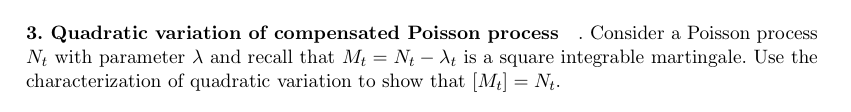
\includegraphics[width=\textwidth]{ex3.png}

\begin{equation*}
Z_t = exp(M_t - \frac{1}{2} [M]_t)
\end{equation*}
For strictly positive processes ln and exp are bijective transformations. We use Ito's formula:
\begin{align*}
exp(ln(Z_t)) &= exp(ln(Z_0) + \int_0^t \frac{1}{Z_s} d Z_s - \frac{1}{2} \int_0^t \frac{1}{(Z_s)^2} d[Z]_s)\\
Z_t &= exp(ln(Z_0) + \int_0^t \frac{1}{Z_s} d Z_s - \frac{1}{2} [\int_0^. \frac{1}{Z_s} d Z_s]_t)
\end{align*}

Integrals with respect to a martingale are martingales. We can therefore conclude that:
\begin{equation*}
M_t = \int_0^t \frac{1}{Z_s} d Z_s
\end{equation*}



%Consider $M$ as an Ito integral $M=\int_0^t \theta_s dW_s$.
%Then we have
%\begin{align*}
%	\qVar{M} &= \qcVar{M}{M} \\
%	&=  \qcVar{\int_0^t \theta_s dW_s}{\int_0^t \theta_s dW_s} \\
%	&= \int_0^t \theta_s^2 d \qcVar{W}{W}_s \\
%	&= \int_0^t \theta_s^2 ds
%\end{align*}
%Therefore
%\begin{align*}
%	exp(M-\frac{1}{2}\qVar{M}) = exp(\int_0^t \theta_s dW_s-\frac{1}{2}\int_0^t \theta_s^2 ds
%) 
%\end{align*}
%Now we can apply Girsanov Thereom and know $exp(M-\frac{1}{2}\qVar{M})$ is a local martingale.   
\end{document}
